\section{Related work}
\label{sec:related_work}
%
Previous work has explored how to visualize volumetric data with lenses and distortion techniques to address occlusion issues. In this context, one major challenge is to maintain a comprehensible embedding of the deformed focus area within its context. Another challenge is to have techniques that operate at truly interactive rates (tens of frames per second), which can be difficult when the deformations are applied to volumetric data rendered by DVR. Related work can be further divided into occlusion management techniques and lenses-and-deformation techniques, as follows.

\subsection{Occlusion management}
%
Many approaches for occlusion management have been proposed\,\cite{4483791}. Multiple viewports, a view paradigm using two or more views, can be used to see the data from different perspectives\,\cite{WangBaldonado:2000:GUM:345513.345271}. However, this does not help when the target is strongly occluded from \emph{all} possible viewpoints. Virtual X-ray methods make targets visible by turning occluders invisible~\cite{Burns:2008:ACC:1457515.1409107} or half-transparent. Kruger et al.~\cite{4015450} proposed ClearView, an interactive technique that enables users to focus on particular areas in the data while preserving context information without visual clutter by modulating the transparency. Correa and Ma~\cite{5416704} proposed visibility-driven transfer functions (TFs) to maximize the visibility of data intervals of interest. Yet, designing good TFs is still challenging in general: For instance, in baggage inspection, a dissimulation strategy is to hide a threat among objects with the same density, case in which one cannot easily remove occluders but keep the target by TF editing\,\cite{xxx}. Similar situations occur when aiming to de-occlude a tumor from surrounding similar-density tissue in medical scans\,\cite{xxx}. For DVR, in addition to removing occluding voxels based on density values and position, Rezk-Salama and Kolb~\cite{CGF:CGF979} also considered the voxels' occurrence on the casted ray. Later, Hurter et al. proposed several lens techniques that remove occluders by deforming (pushing them away) in a focus area, applicable to 2D images, multivariate volumes, and trail sets~\cite{moleview,6787171}. However, such techniques rely on the specification of occluders based on data value-ranges, thus share limitations with ClearView and related techniques. Li et al.~\cite{Li:2012:LVV:2425296.2425325} proposed a system for baggage visualization where occluded objects are clarified by moving away occluders via an interactive process called virtual unpacking. However, this technique severely alters the \emph{context} in which the occluder occurs, by altering or removing potentially important information, \emph{e.g.}, relative position and connectivity -- a clearly unwanted proposition in \emph{e.g.} medical contexts. Recently, an interactive visualization system was proposed for volumetric data exploration with direct manipulation of voxels\,\cite{7819413}. However, extending such approaches in a DVR setting to more complex deformations or changes of the data in focus is computationally challenging.

\begin{figure*}[htbp]
\centering
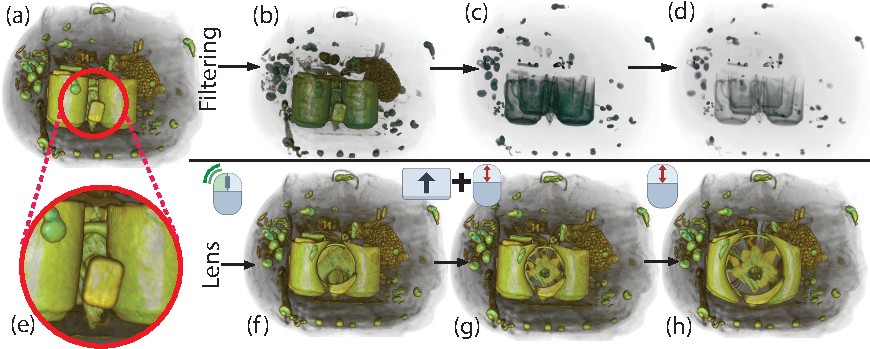
\includegraphics [width=0.7\textwidth]{shuriken.pdf}
\vspace{-0.15cm}
\caption{(a) A suspicious object is spotted between a set of mugs. (b)-(d) Filtering densities using a classical 1D transfer function removes progressively more of the occluders (mugs), but also removes the target. (e) The user applies the lens on the target object (double-click). An animation starts opening the lens. Halfway the animation, the object is magnified, but only the area close to the lens is visible. (f) The fish-eye field of view at the end of the animation fully shows the target. (g) The lens is increased to magnify the target (mouse scroll).}
\label{f:baggage_lens}
\end{figure*}
\vspace{-0.15cm}

\subsection{Lenses and deformations}
%
An interactive lens is a lightweight tool to solve a localized visualization problems by temporarily altering a selected part of the visual representation of the data\,\cite{CGF:CGF12871}. In other words, a lens is a parameterizable selection according to which a base visualization is altered. These property are very effective for providing focus-and-context (F+C) solutions to occlusion in volumetric data. Parametrizable properties of a lens include the position, shape, appearance, size, orientation, and selection of the included data (focus). The \emph{shape} of a lens is usually chosen to fulfill the requirements of the application and is strongly linked to the lens function. Most lenses are circular\,\cite{1648236} or rectangular\,\cite{Kincaid:2010:SFA:1907651.1907963}. Our lens has also a circular shape in order to remind its magnifying property. Some lenses, such as the JellyLens~\cite{Pindat:2012:JCA:2380116.2380150} and the smart lenses~\cite{Thiede2008}, can adapt their shape automatically to the focus data. Modifying the lens \emph{position} and/or \emph{size} sets its focus on a different part of the data according to the user's interest. One can automatically update position and size to guide the user toward interesting events in the data\,\cite{Tominski:2011:ECU:2336207.2336211} or guide the exploration path along interesting events\,\cite{Alvina:2014:RER:2598153.2598200}. In this sense, our lens updates automatically its properties once a target has been selected. This allows a smooth transition towards an unobstructed and magnified area of interest.

Lenses for volume visualization face challenges mainly related to spatial selection and occlusion. Wang et al. address these issues by proposing the Magic Lens\,\cite{1532818}, which renders the occlusions with higher transparency and magnifies volumetric pre-computed features interactively or automatically in a pre-segmented dataset. In addition to interactively magnifying areas of interest, our lens frees them from obstruction and allows local modification of the viewpoint, lighting, and TF, to offer many exploration perspectives. Tong et al. proposed the GlyphLens~\cite{7539643} that removes occluding glyphs by pulling them aside through animation. While effective, this technique addressed only 3D glyph-based volumetric visualizations. Lenses can create discontinuities between their inner part and the rest of the volume. Deformation can be a solution to this discontinuity issue.

To increase the flexibility of deformation, Hsu et al. developed a framework that uses non-linearly sampled rays to smoothly project objects in a scene at multiple levels of detail onto a single image\,\cite{Hsu:2011:RFM:2070781.2024165}. However, this technique requires significant computational effort to render a single image from features of interest at different scales. Bruckner and  Groller~\cite{4015467} proposed exploded views for volume data by partitioning the volume into several segments. Correa et al. proposed a framework\,\cite{Correa:2007:IDD:1313046.1313163} allowing  users to physically manipulate the geometry of a data object. McGuffin et al.\,\cite{1250400} performed deformations using peeling to see hidden parts of the data. In general, these techniques have the disadvantage of removing potentially important contextual information surrounding the target when trying to solve the local occlusion.

Deformations can reveal predefined features in the data by taking into account a precomputed segmentation. Tong et al. proposed a deforming lens which moves streamlines to observe the inner part of streamline bundles\,\cite{7332955}. Other techniques performed deformations using surgical metaphors\,\cite{4069230,Correa:2006:FAV:1187627.1187827} to show hidden parts of a volume. Such techniques do not offer tools for local manipulation of the viewpoint that allows seeing a target under multiple perspectives while keeping the global context. To this end, our lens proposes an interactive volume deformation based on GPU accelerated ray-casting to free a designated target from local occlusion while keeping the global context.

\subsection{Contributions}
%
Summarizing the above, we propose a new technique which combines high-quality DVR with a fast, versatile, and easy to use, lens to support the interactive visualization of occluded data in volumes. According to the classification of view deformations by Carpendale et al.~\cite{595268}, we use a nonlinear radial distortion through an interactive lens to remove occluding items and keep the global context while magnifying a partially occluded item. Within the body of work on volumetric lens techniques, we frame our contribution as follows:
\begin{itemize}
\item we propose an interactive deforming lens that magnifies and pushes aside occluding objects located in front of a designated focal point at an interactive frame-rate. For this, we propose a GPU-accelerated raycasting scheme able to compute ray deformations;
\item we allow flexible and real-time interactive modification of the focal point, custom bent rays used for DVR, lens deformation, and shading and transfer function in the focus area. Combined, these allow us to provide \emph{on the fly} a range of perspectives of the objects in focus, that is, without having to change the viewpoint or manipulate complex parameters in linked views.
\end{itemize}


